\documentclass[a4paper]{article}
\usepackage[english]{babel}
\usepackage[utf8x]{inputenc}
\usepackage{tikz}
\usepackage{tabu}
\usepackage{courier}
\usepackage{graphicx}
\usepackage{listings}
\usepackage{caption}
\usepackage{subcaption}
\usepackage{float}
\title{CSC 214 Final Project Proposal}
\author{Nate Conroy}

\begin{document}

\maketitle

\section{General Overview}

For my final project for CSC 214, I intend to make an app that caters to the local music scene in cities where the app is used. The app will be categorized as an event sharing app, where users can create an account as a fan, as a band manager, or as a venue owner, and can post geotagged events for upcoming shows at local venues in order to spread the word, or find other bands to play with.

The inspiration for this app came from a real-world dilemma that my band faced as a part of the local music scene in Syracuse, NY. We found that it was tough to connect with other bands in the area in order to organize shows without jumping around many different Facebook groups and other websites to listen to some of the bands' material.

\section{Functionality}

The app will have a main event feed that can be filtered in several different ways. The main feature being geographic location. Some other ideas at this time are also filtering by genre of music, and by the "fullness" of an event (is the bill full or is the event organizer looking for more musicians to add).

Events can be created by any user, and will contain information about the date of the show, the venue and its location, the bands listed to perform, the cost/pay, and possibly some other information.

Clicking on a band or artist's name anywhere in the app will launch their page, which will contain a basic bio, as well as some sample music which can be played, and their upcoming events.

Clicking on a venue's name anywhere in the app will launch its page, which will contain some basic information, including photos and a map which will pinpoint the location of the venue.

\subsection{Advanced Features}

The app will utilize the following advanced features:

\begin{itemize}
  \item The ability to use a camera to take photographs (band pages)
  \item Playing sounds with sound pool (transition effects)
  \item Playing longer sounds with MediaPlayer (sample music on band pages)
  \item Google maps services (venue location, setting feed radius from events)
  \item Either network connectivity or recording video (may attempt network connectivity, but if it becomes too much work for this time frame I will use video)
\end{itemize}

\section{Mockups}

\begin{figure}[H]
  \centering
  \begin{minipage}[b]{0.85\textwidth}
    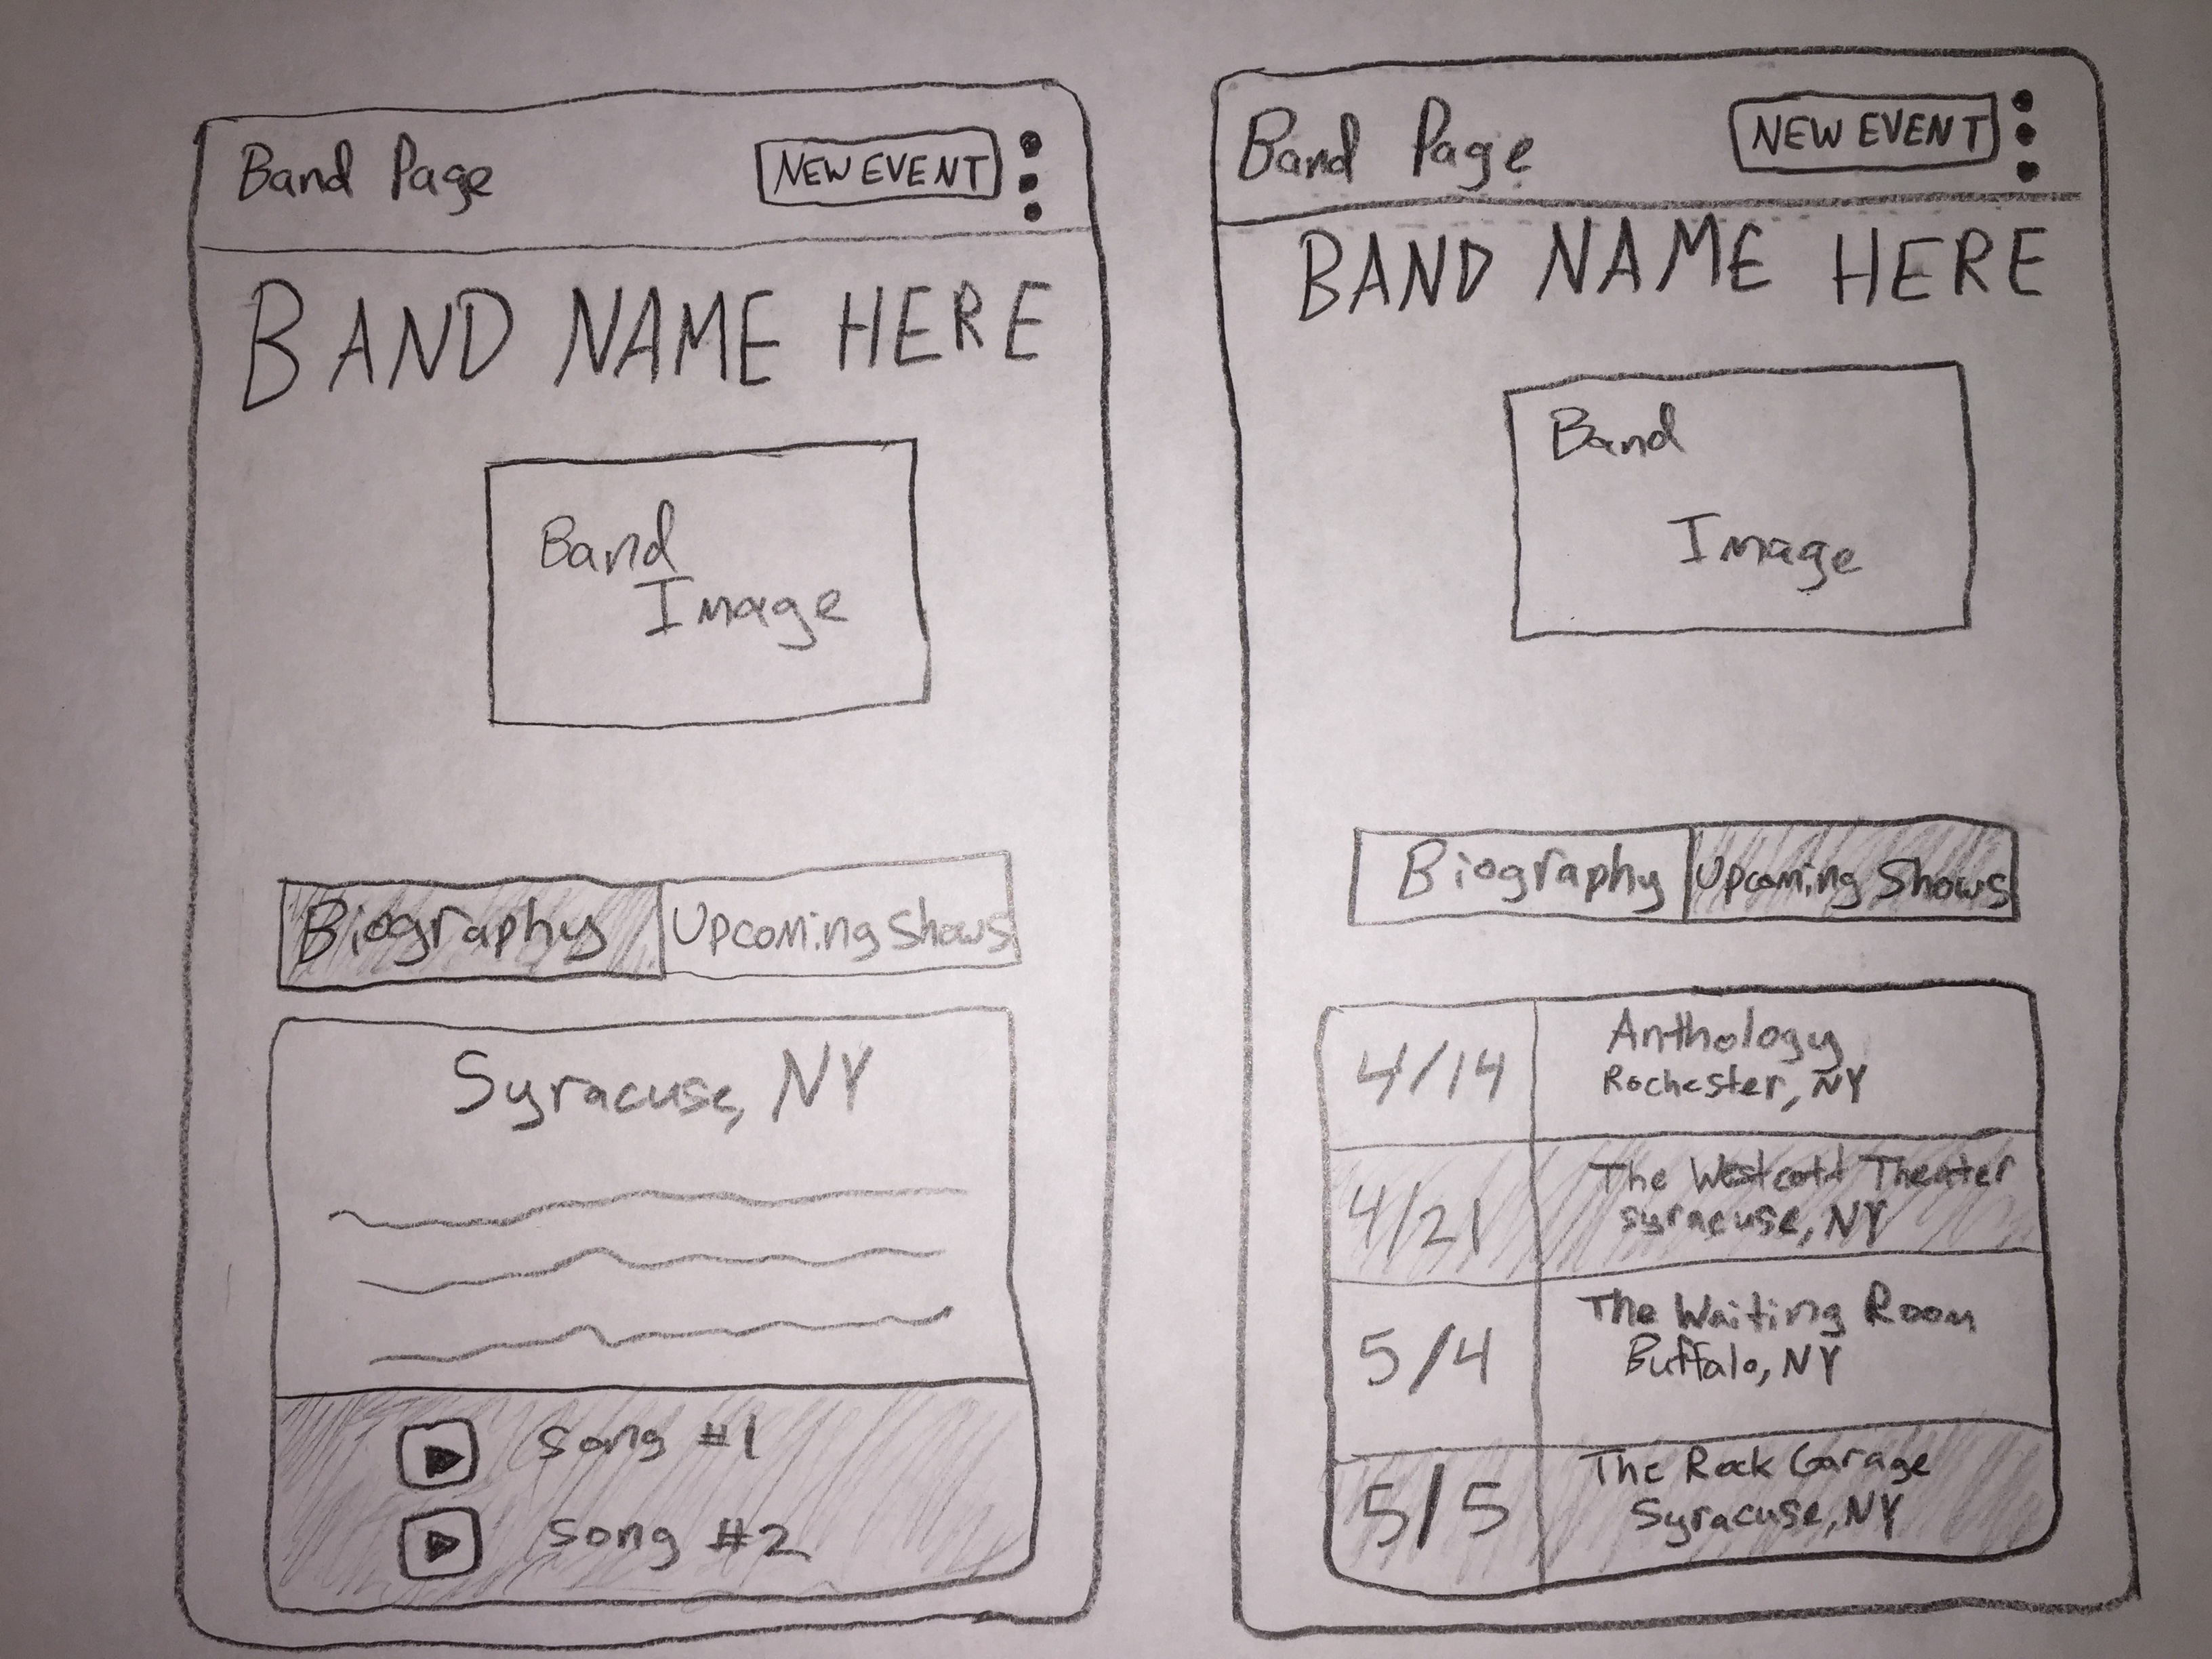
\includegraphics[width=\textwidth]{band_page.jpg}
    \caption{band page}
  \end{minipage}
\end{figure}

\begin{figure}[H]
  \centering
  \begin{minipage}[b]{0.5\textwidth}
    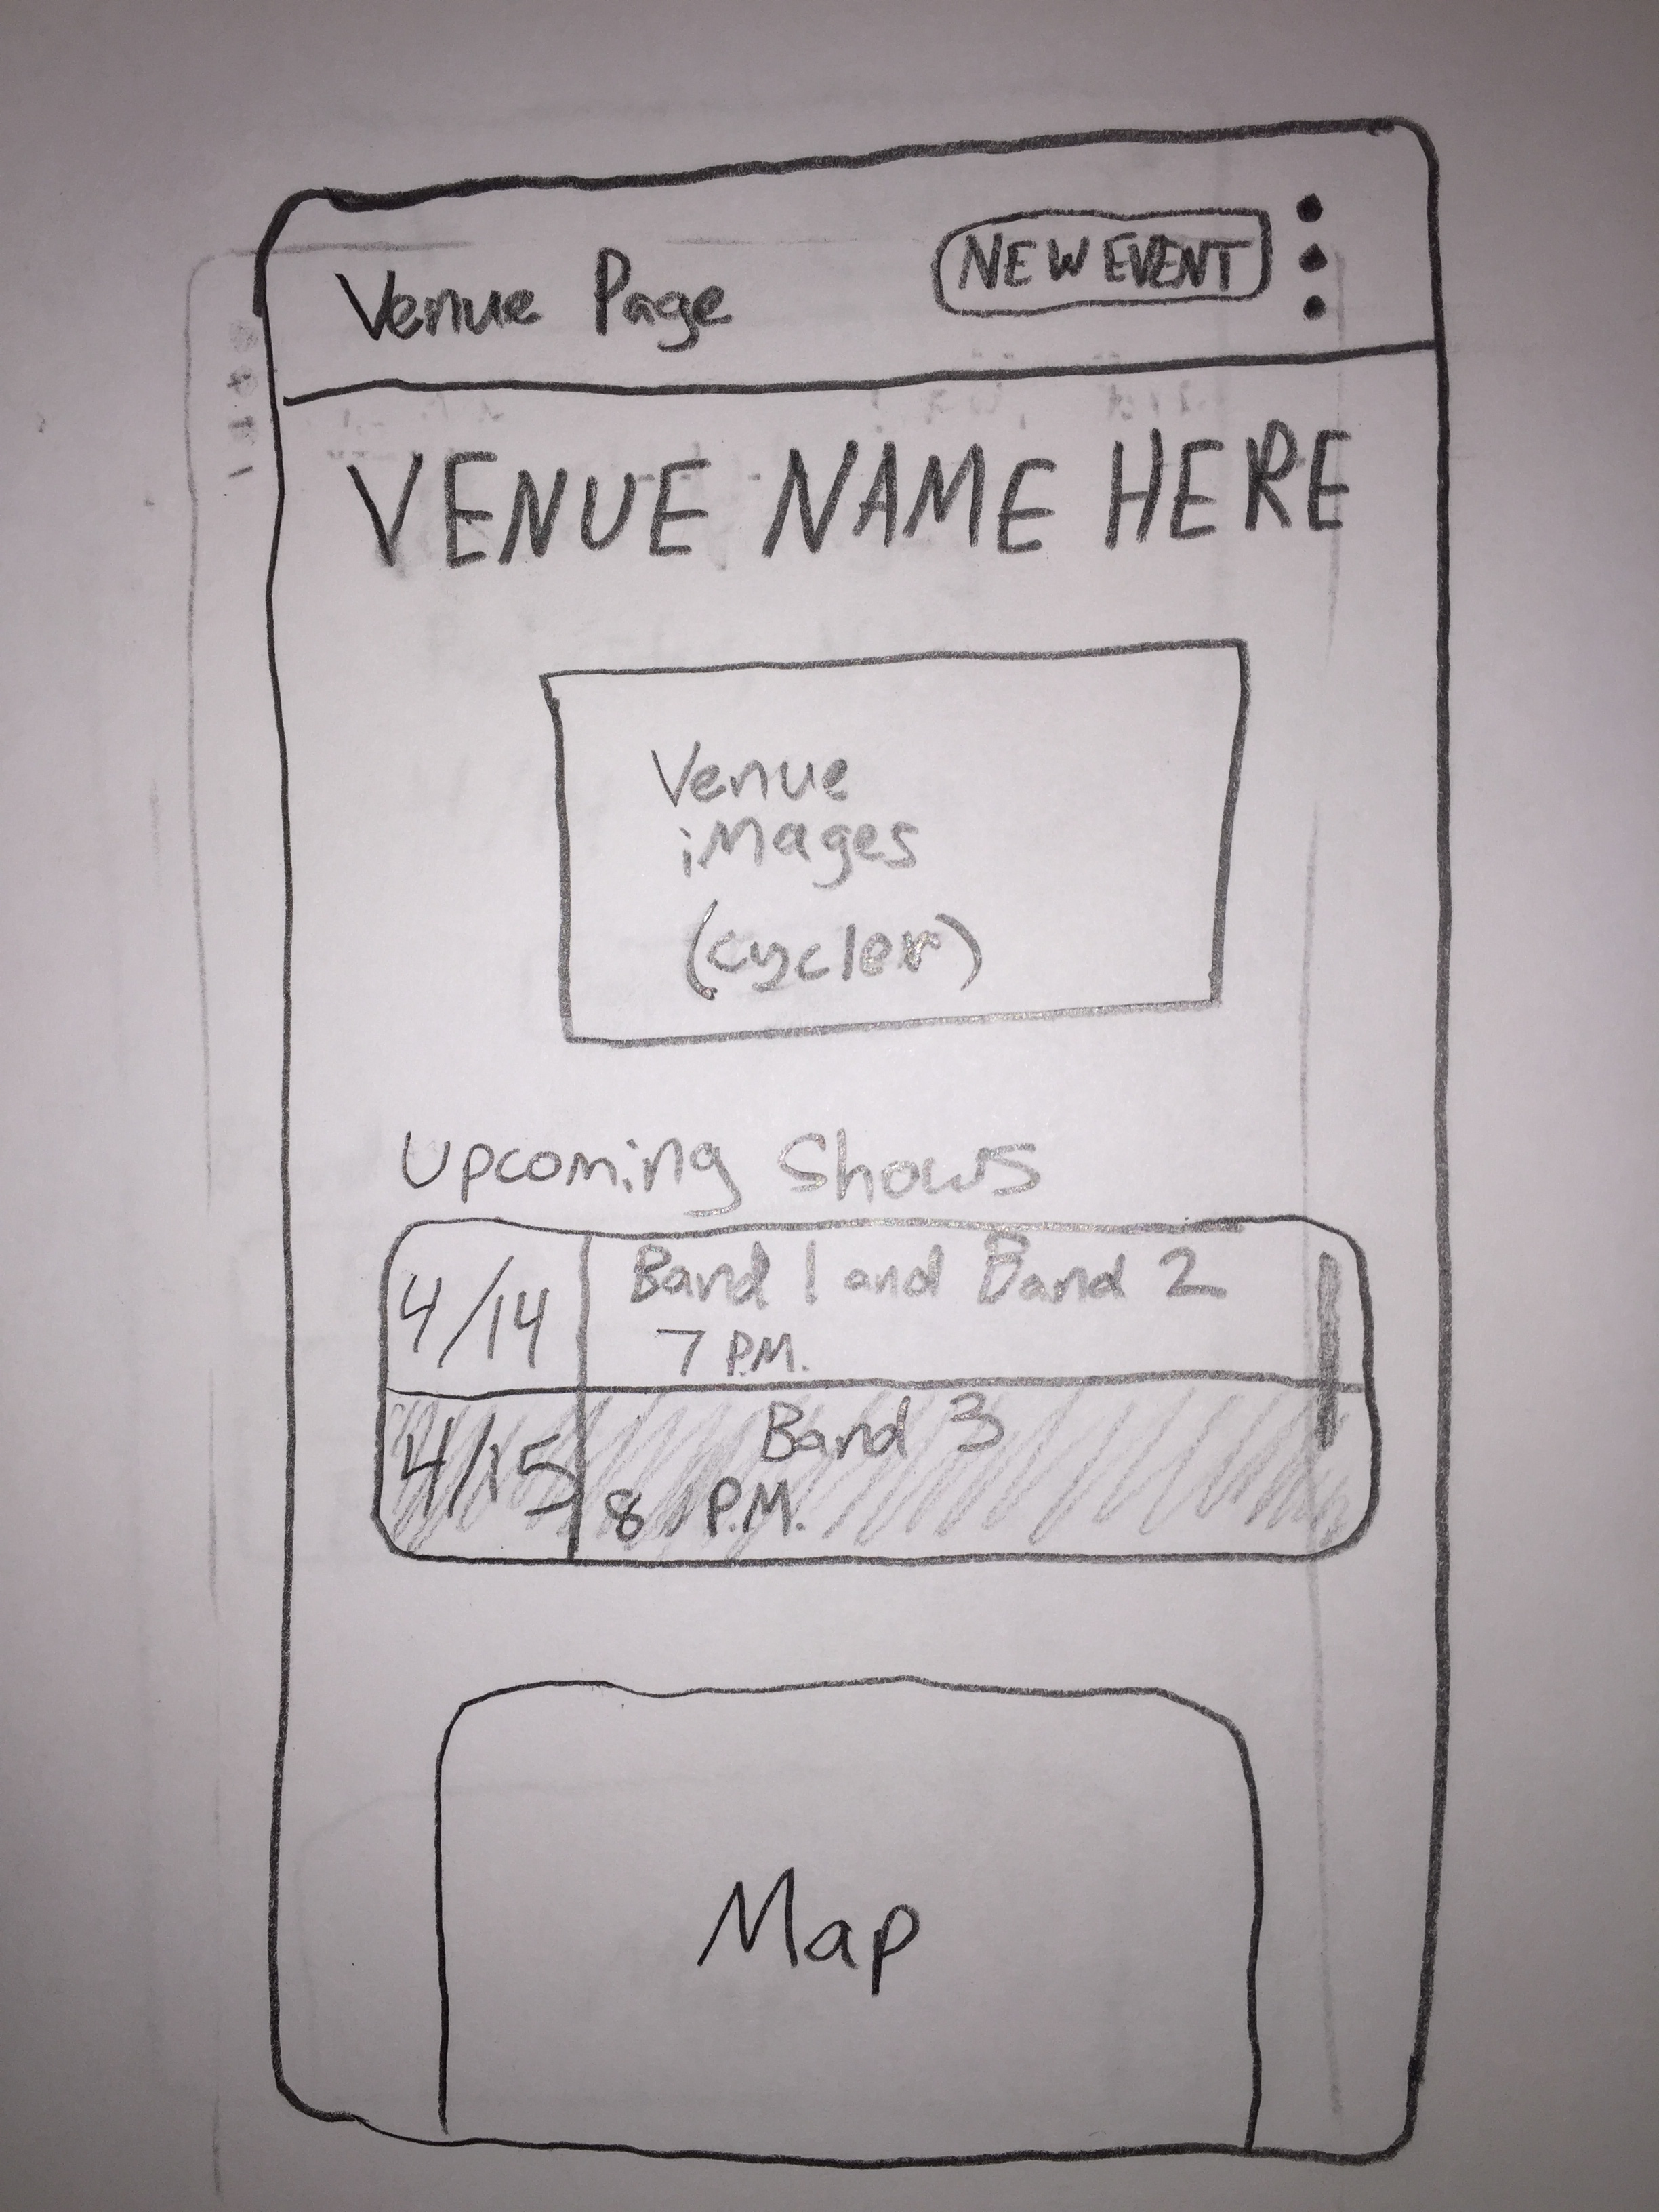
\includegraphics[width=\textwidth]{venue_page.jpg}
    \caption{venue page}
  \end{minipage}
\end{figure}

\begin{figure}[H]
  \centering
  \begin{minipage}[b]{0.5\textwidth}
    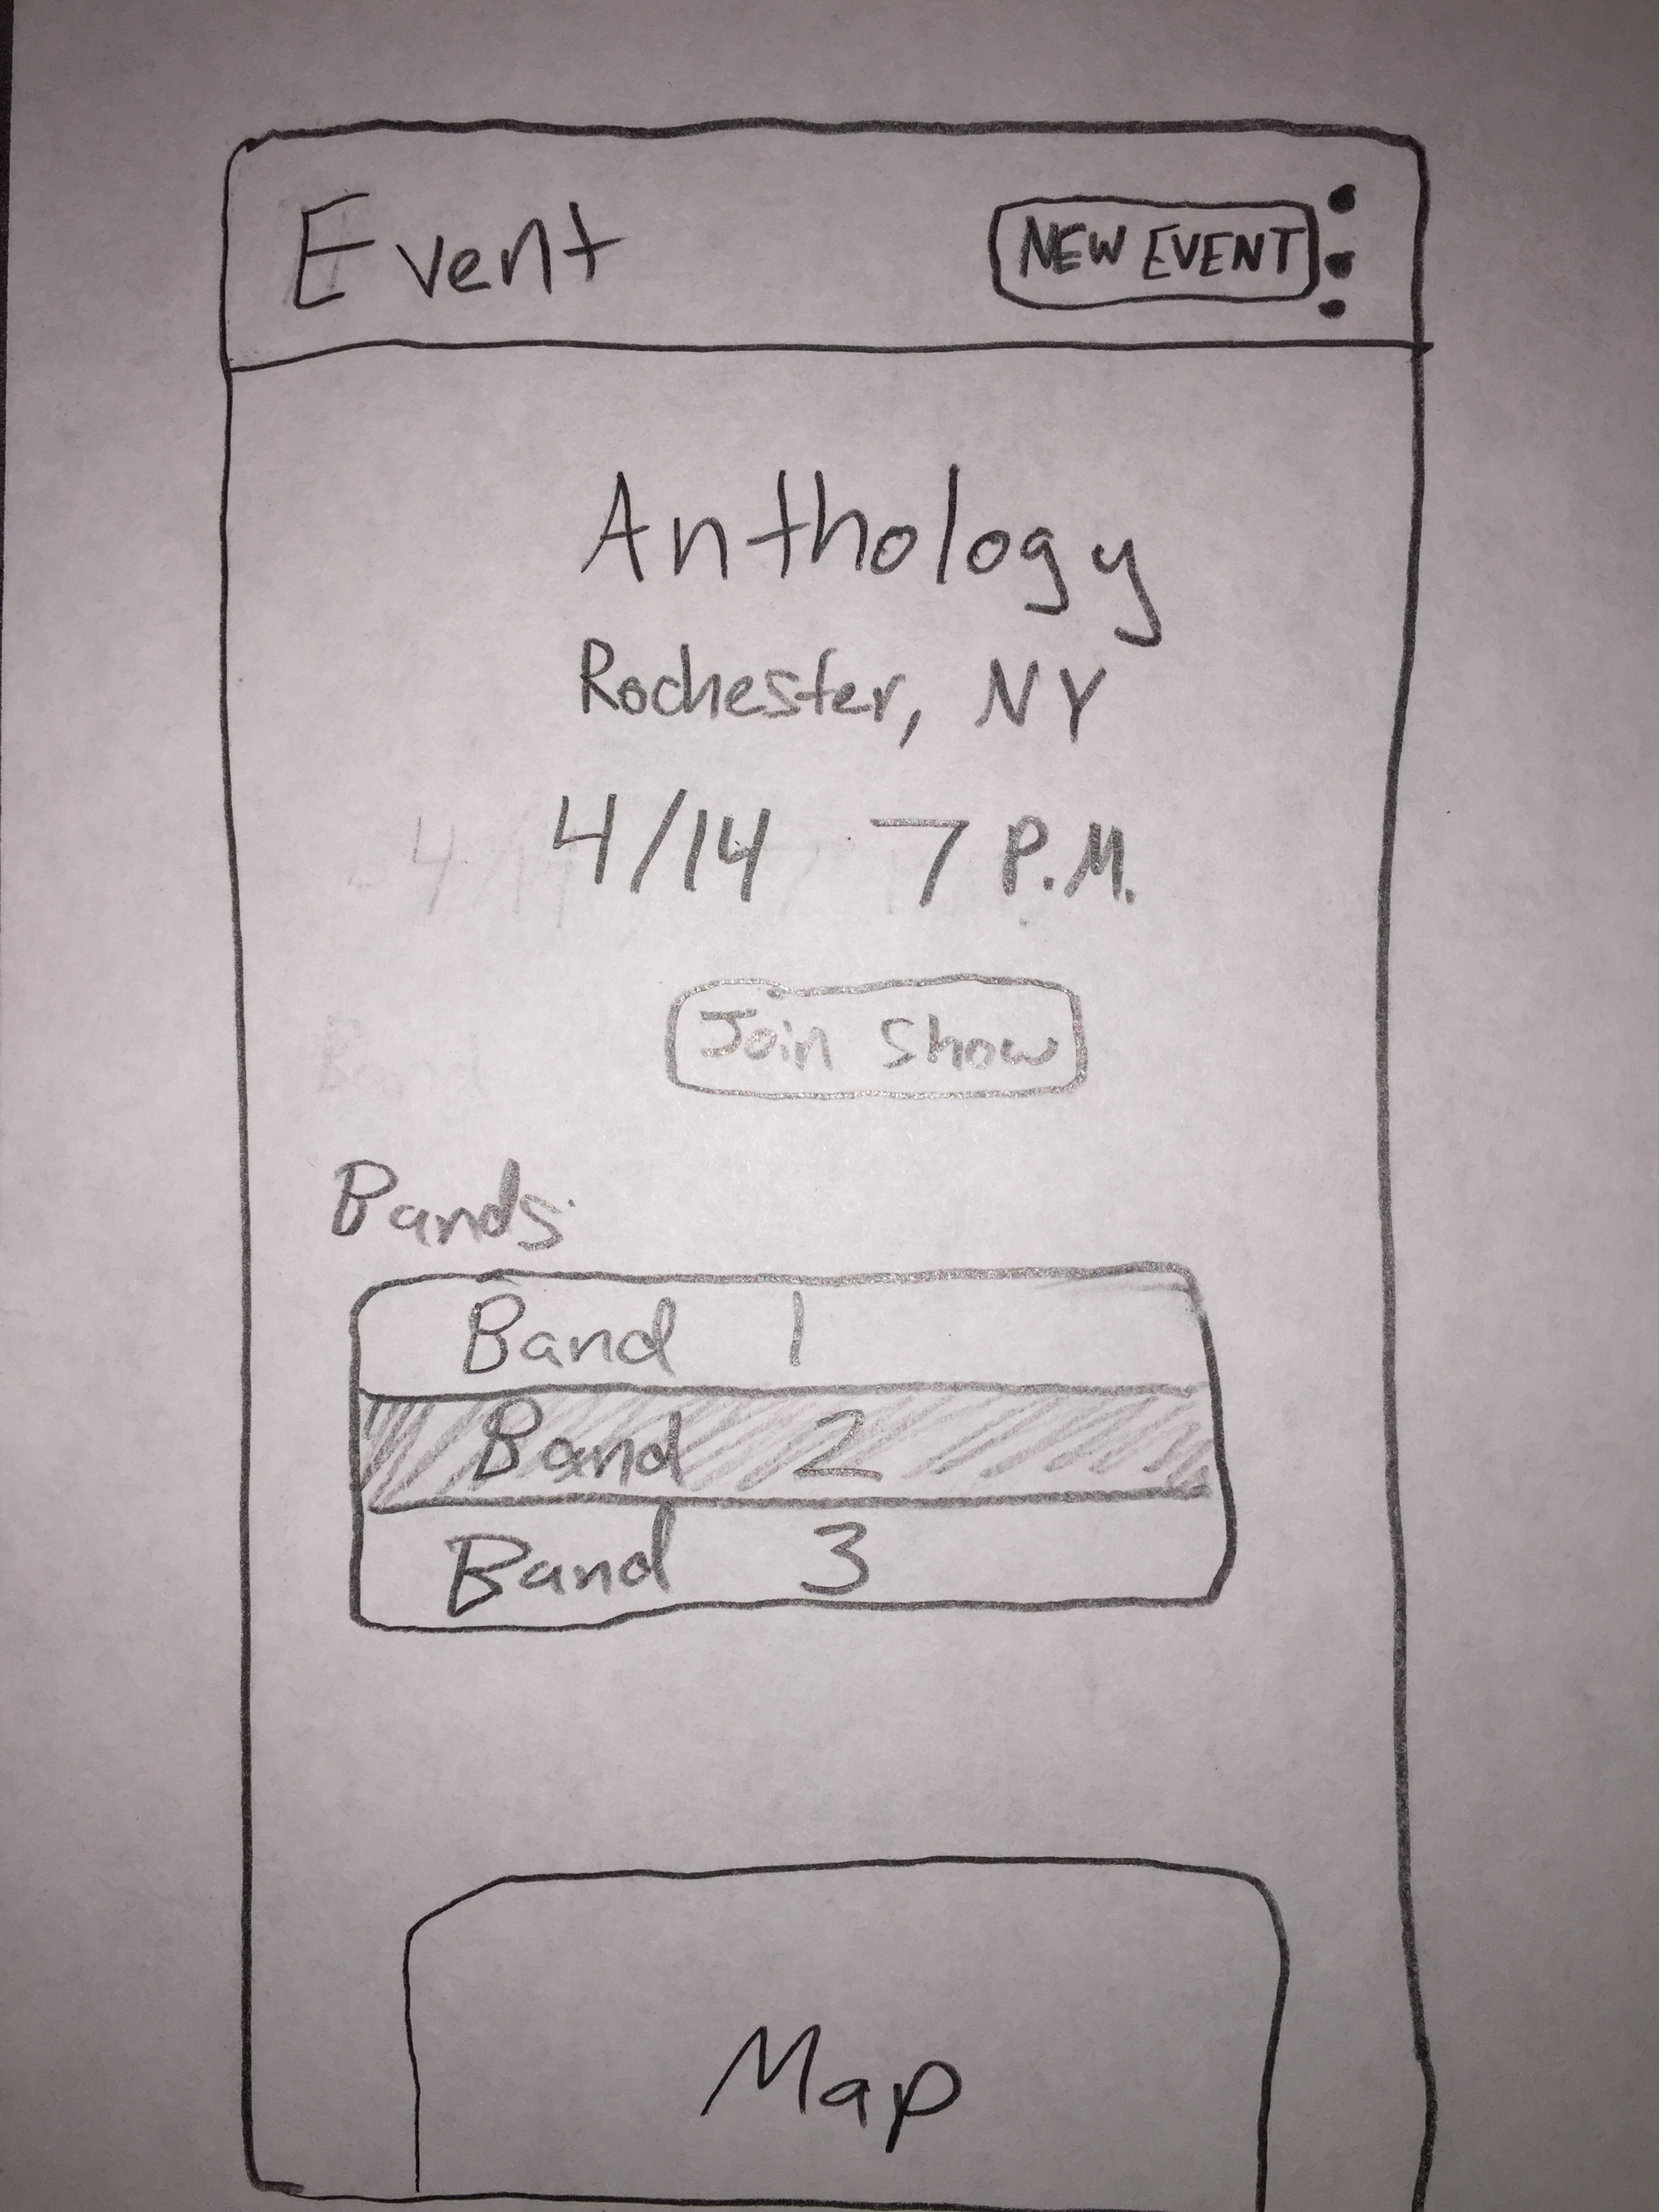
\includegraphics[width=\textwidth]{event_page.jpg}
    \caption{event page}
  \end{minipage}
\end{figure}

\begin{figure}[H]
  \centering
  \begin{minipage}[b]{0.5\textwidth}
    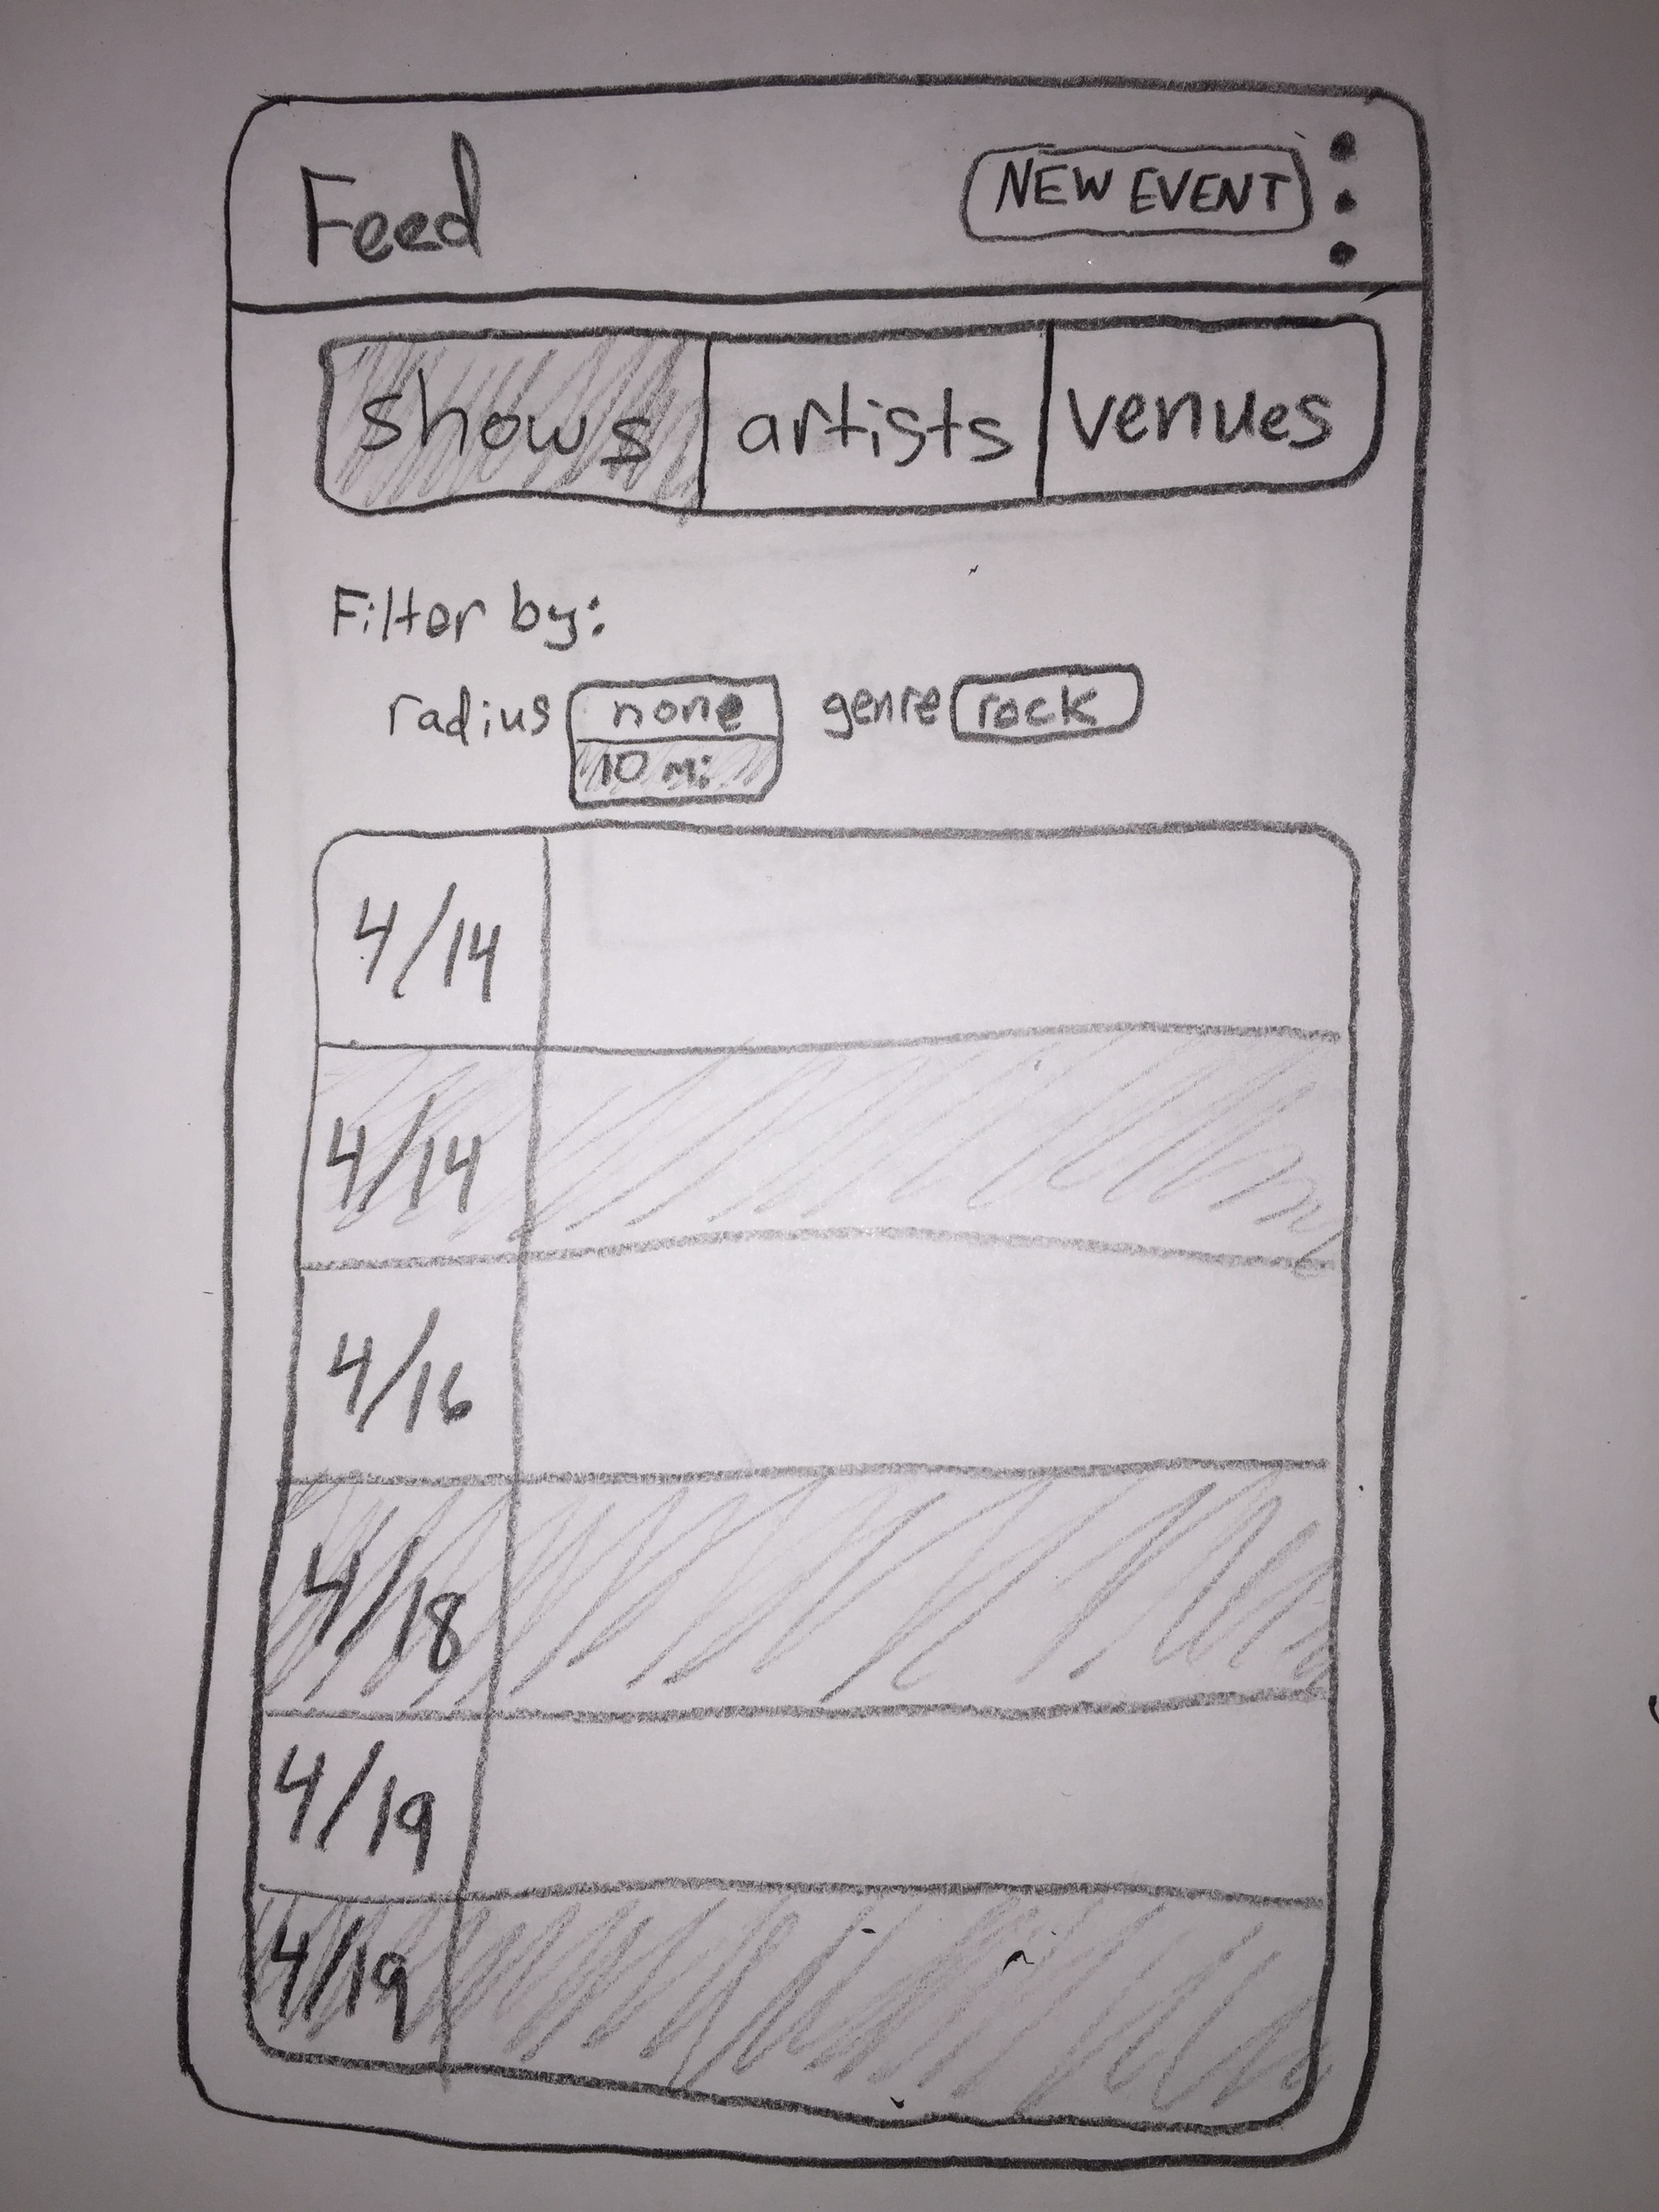
\includegraphics[width=\textwidth]{feed.jpg}
    \caption{feed}
  \end{minipage}
\end{figure}

\begin{figure}[H]
  \centering
  \begin{minipage}[b]{0.85\textwidth}
    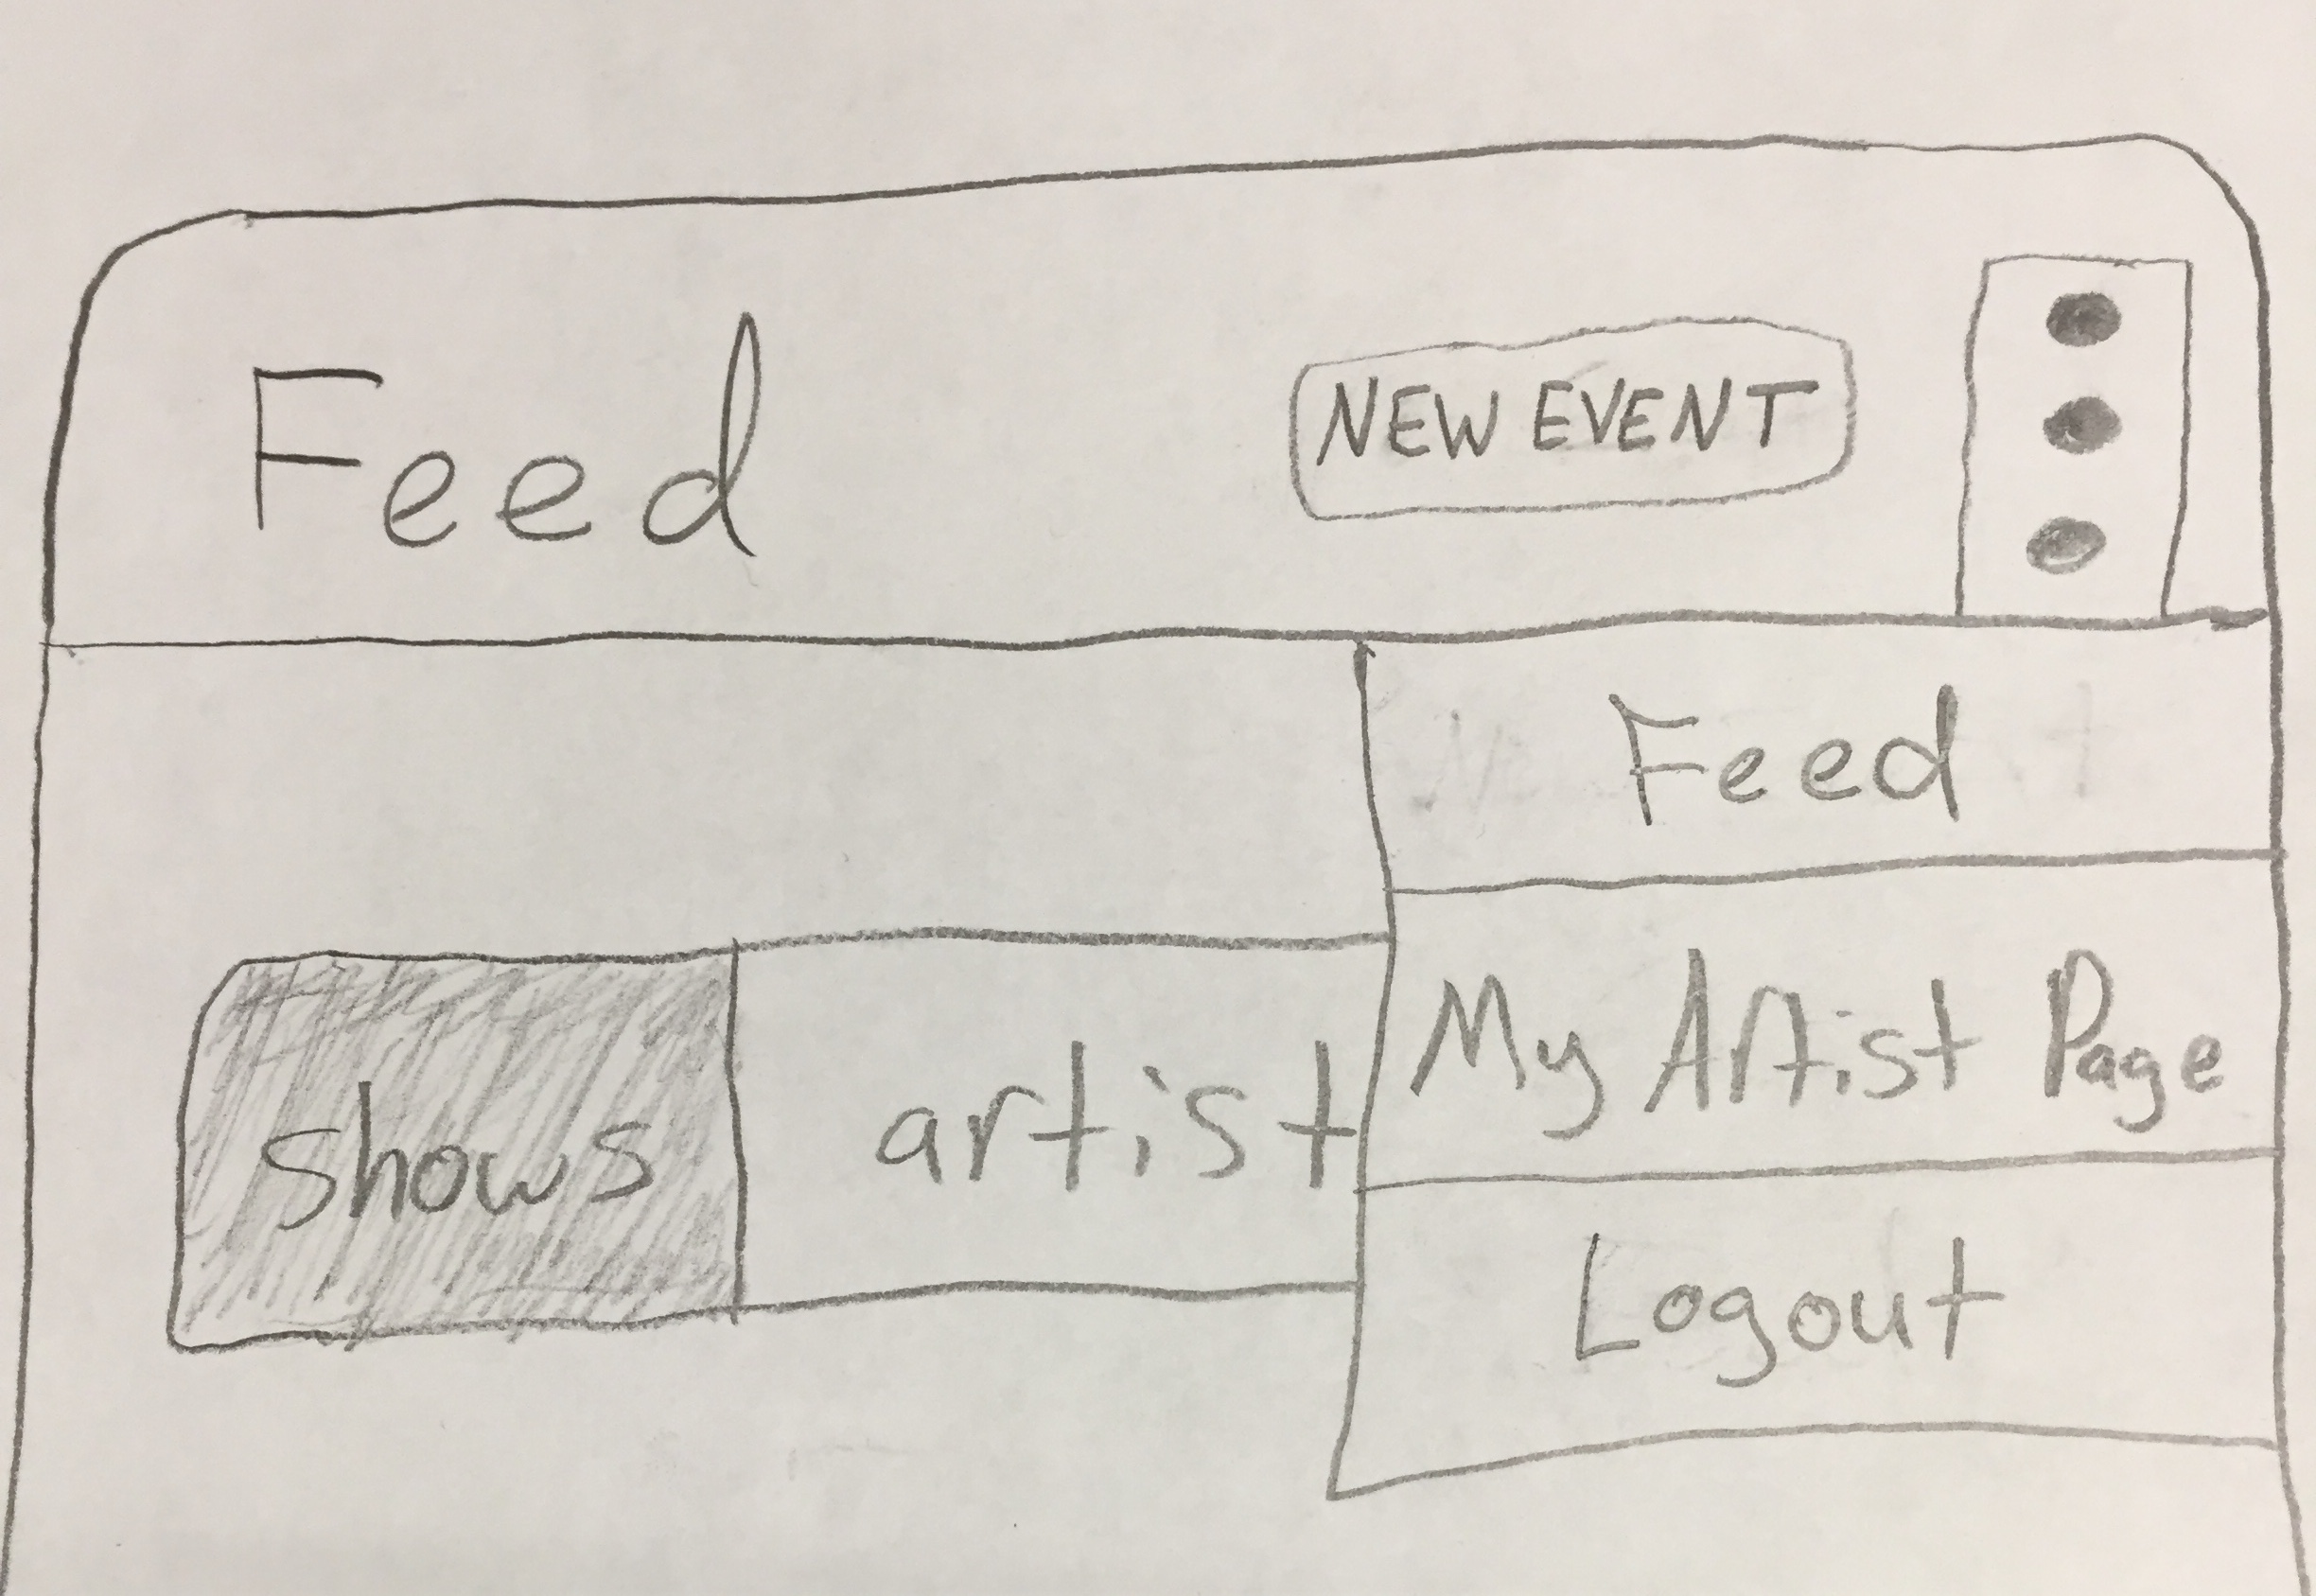
\includegraphics[width=\textwidth]{menu.jpg}
    \caption{menu}
  \end{minipage}
\end{figure}

\end{document}